%%%%%%%%%%%%%%%%%%%%%%%%%%%%%%%%%%%%%%%%%
% Stylish Article
% LaTeX Template
% Version 2.1 (1/10/15)
%
% This template has been downloaded from:
% http://www.LaTeXTemplates.com
%
% Original author:
% Mathias Legrand (legrand.mathias@gmail.com) 
% With extensive modifications by:
% Vel (vel@latextemplates.com)
%
% License:
% CC BY-NC-SA 3.0 (http://creativecommons.org/licenses/by-nc-sa/3.0/)
%
%%%%%%%%%%%%%%%%%%%%%%%%%%%%%%%%%%%%%%%%%

%----------------------------------------------------------------------------------------
%	PACKAGES AND OTHER DOCUMENT CONFIGURATIONS
%----------------------------------------------------------------------------------------

\documentclass[fleqn,10pt]{SelfArx} % Document font size and equations flushed left

\usepackage[english]{babel} % Specify a different language here - english by default

\usepackage{lipsum} % Required to insert dummy text. To be removed otherwise
\usepackage[bookmarks=true,pdfborder={0 0 0}]{hyperref}
\hypersetup{colorlinks=TRUE,linkbordercolor=red,linkcolor=green,pdfborderstyle={/S/U/W 1}}
\usepackage{amsmath} 
\usepackage{textcomp}
\usepackage{url}



%----------------------------------------------------------------------------------------
%	COLUMNS
%----------------------------------------------------------------------------------------

\setlength{\columnsep}{0.55cm} % Distance between the two columns of text
\setlength{\fboxrule}{0.75pt} % Width of the border around the abstract

%----------------------------------------------------------------------------------------
%	COLORS
%----------------------------------------------------------------------------------------

\definecolor{color1}{RGB}{0,0,90} % Color of the article title and sections
\definecolor{color2}{RGB}{0,20,20} % Color of the boxes behind the abstract and headings

%----------------------------------------------------------------------------------------
%	HYPERLINKS
%----------------------------------------------------------------------------------------

\usepackage{hyperref} % Required for hyperlinks
\hypersetup{hidelinks,colorlinks,breaklinks=true,urlcolor=color2,citecolor=color1,linkcolor=color1,bookmarksopen=false,pdftitle={Title},pdfauthor={Author}}

%----------------------------------------------------------------------------------------
%	ARTICLE INFORMATION
%----------------------------------------------------------------------------------------

\JournalInfo{Data Mining B565 Fall 2016} % Journal information
\Archive{} % Additional notes (e.g. copyright, DOI, review/research article)

\PaperTitle{House Prices: Advanced Regression Techniques} % Article title

\Authors{Ankit Saxena, Samvat Rastogi, Shailendra Patil} % Authors

\Keywords{Data Mining --- Kaggle ---  Housing --- Regression --- Prediction} % Keywords - if you don't want any simply remove all the text between the curly brackets
\newcommand{\keywordname}{Keywords} % Defines the keywords heading name

%----------------------------------------------------------------------------------------
%	ABSTRACT
%----------------------------------------------------------------------------------------

\Abstract{This project deals with predicting the Sales Price of individual residential properties in Ames, Iowa. The data set consists of 'Training Data' and 'Test Data'. The goal is to generate an appropriate regression model using the 'Training Data' and then predict the Sales Price for the given 'Test Data' based on the generated model. The 'Training Data' consists of 1460 observation and 81 Attributes including the Sales Price and 'Test Data' contains 1459 observations with 80 attributes which does not include Sales Price. Before applying any model, the data is preprocessed to take care of missing values and also to reduce number of attributes being used for model training. After data preprocessing, various regression methods like Linear Regression, Random Forest, Gradient Boosting, Extreme Gradient Boosting are applied and compared. Then, the model with the least error rate is used to predict the Sales Price of the houses using 'Test Data'.}

%----------------------------------------------------------------------------------------

\begin{document}

\flushbottom % Makes all text pages the same height

\maketitle % Print the title and abstract box

\tableofcontents % Print the contents section

\thispagestyle{empty} % Removes page numbering from the first page

%----------------------------------------------------------------------------------------
%	ARTICLE CONTENTS
%----------------------------------------------------------------------------------------

\section*{Introduction} % The \section*{} command stops section numbering
"The Housing Market refers to the supply and demand for houses, usually in a particular country or region. A key element of the housing market is the average house prices and trend in house prices \cite{REF:1}. For many people buying a property is one of the important decisions in life. There are many factors like Area, Neighborhood, Connectivity, Transportation, House Price, etc. that impacts this decision.
\\ Hence, it becomes very important to know the trend in which the houses are being sold, so that as a buyer we might have a rough idea what can be the expected price of a house. Predictive analysis is what is required here. As an analyst, we build various model and predict the rough estimate of the prices, which might be used by the property evaluators for their clients.

\addcontentsline{toc}{section}{Introduction} % Adds this section to the table of contents

%------------------------------------------------

\section{Data}


%\begin{equation}
%\cos^3 \theta =\frac{1}{4}\cos\theta+\frac{3}{4}\cos 3\theta
%\label{eq:refname2}
%\end{equation}

\subsection{Data Background}
The data that has been provided for analysis consists of 3 files
\begin{enumerate}[noitemsep]
\item \textbf{train.csv}
\item \textbf{test.csv}
\item \textbf{data$\_$description.txt}
\end{enumerate}

Training and Test data files consists of a column named ID, which can be used to uniquely identify every house and there are 79 features that can be used to predict the Sales Price of the house. Training data file consists of an additional column named Sale Price. The regression models have been developed on the training data to predict the value of Sales Price of the Test data. The data$\_$description file provides all the necessary information regarding the attributes.
The data was downloaded from Kaggle \cite{REF:8}.


\subsection{Data Description}
The training data has 78 attributes excluding the ID and Sales Price and a total of 1460 records. The test data has 78 attributes excluding the ID and a total of 1459 records.
Data consists of \textbf{43 categorical features} and \textbf{36 numerical features}. 
\\ \\ The \textbf{categorical features} are: MSZoning, Street, Alley, LotShape, LandContour, Utilities, LotConfig, LandSlope, Neighborhood, Condition1, Condition2, BldgType, HouseStyle, RoofStyle, RoofMatl, Exterior1st, Exterior2nd, MasVnrType, ExterQual, ExterCond, Foundation, BsmtQual, BsmtCond, BsmtExposure, BsmtFinType1, BsmtFinType2, Heating, HeatingQC, CentralAir, Electrical, KitchenQual, Functional, FireplaceQu, GarageType, GarageFinish, GarageQual, GarageCond, PavedDrive, PoolQC, Fence, MiscFeature, SaleType, SaleCondition.
\\ \\The \textbf{numerical features} are: MSSubClass, LotFrontage, Lot Area, OverallQual, OverallCond, YearBuilt, YearRemodAdd, MasVnrArea, BsmtFinSF1, BsmtFinSF2, BsmtUnfSF, TotalBsmtSF, X1stFlrSF, X2ndFlrSF, LowQualFinSF, GrLivArea, BsmtFullBath, BsmtHalfBath, FullBath, HalfBath, BedroomAbvGr, KitchenAbvGr, TotRmsAbvGrd, Fireplaces, GarageYrBlt, GarageCars, GarageArea, WoodDeckSF, OpenPorchSF, EnclosedPorch, X3SsnPorch, ScreenPorch, PoolArea, MiscVal, MoSold, YrSold.


\subsection{Data Preprocessing}
The biggest task in any Data Mining problem is Data Preprocessing. Before we apply any algorithms, we first need to clean the data. The data might contain missing values, outliers, etc. There could be different kinds of attributes in the given data, like continuous variables, categorical variables, nominal, ordinal, ranges, ratios, etc. Such variables need to be taken care of based on the model we want to apply. Data preprocessing not only deals with these thing but also covers feature selection, data reduction, etc. Given a set of attributes, not every attribute is important for data analysis or prediction. Few attributes might be of no use and few attributes will be very vital for our analysis. For this purpose we do feature selection.


\subsubsection{Missing Data Imputation}
There are many attributes which have NA (Not Applicable) as one of the accepted value in their domain. These NA\textquotesingle s are not missing values but rather explain the absence of a particular feature in the house. The following attributes have NA in their domain:
Alley, BsmtQual, BsmtCond, BsmtExposure, BsmtFinType1, BsmtFinType2, FireplaceQu, GarageType, GarageFinish, GarageQual, GarageCond, PoolQC, Fence, MiscFeature.
\\ The NA values for these attributes were replaced with \textbf{NC} while cleaning the data, to differentiate the actual missing values for other attributes with these 14 attributes.
\\ \\ After replacing the NA values with NC for these attributes, we found the actual number of NA values or missing values.
A total of \textbf{357} values are missing in the Training data.
A total of \textbf{358} values are missing in the Test data.
The percentage of missing values in the training data is 0.3018\%.
The percentage of missing values in the test data is 0.3067\%.
\\ \\The majority of values are missing for the attribute LotFrontage.
The percentage of missing values for LotFrontage in training data is 17.739\%.
The percentage of missing values for LotFrontage in test data is 15.558\%.
The mean of the values for attribute LotFrontage in training data is 70.05 and the median is 69.00.
The mean of the values for attribute LotFrontage in test data is 68.58 and the median is 67.00.
Thus, the missing values have been replaced with the mean of the existing values for LotFrontage, as there is not a huge difference between the mean and the median.
\\ \\The attribute GarageYrBlt has the second highest number of missing values.
The percentage of missing values for GarageYrBlt in training data is 5.547\%.
The percentage of missing values for GarageYrBlt in test data is 5.346\%.
The mean of the values for attribute GarageYrBlt in training data is 1979 and the median is 1980.
The mean of the values for attribute GarageYrBlt in test data is 1978 and the median is 1979.
Thus, the missing values have been replaced with the mean of the existing values for GarageYrBlt, as there is not a huge difference between the mean and the median.
\\ \\ Similarly for all other numerical attributes, the missing values were replaced by either mean or median based on the data and for categorical attributes the missing values were replaced by the mode value of that particular attribute.
%\begin{figure}[ht]\centering
%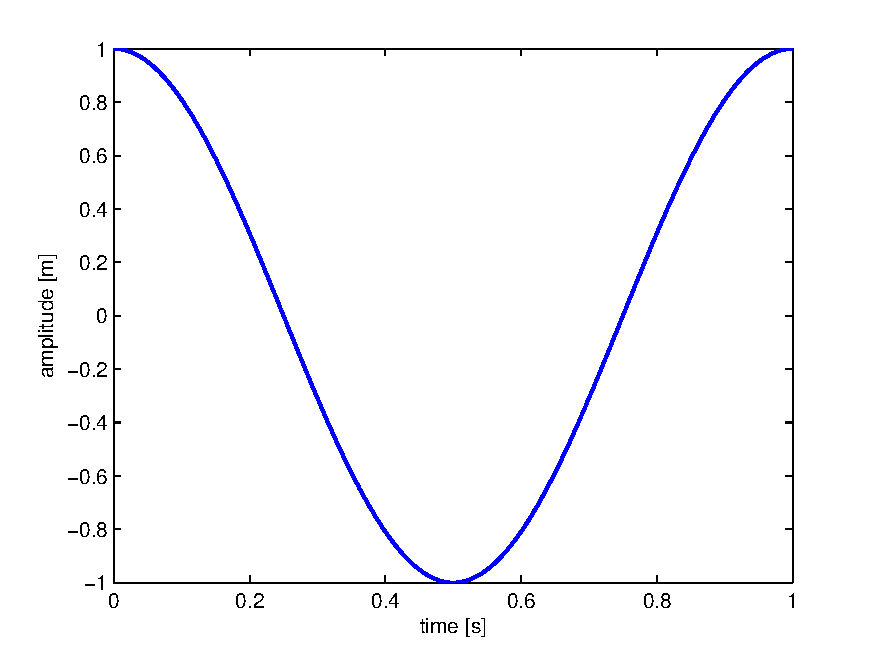
\includegraphics[width=\linewidth]{results}
%\caption{In-text Picture}
%\label{fig:results}
%\end{figure}
%
%Reference to Figure \ref{fig:results}.

%------------------------------------------------
\subsubsection{Outlier Analysis}
Outlier is an observation that diverges from the overall pattern in the sample. In any data, outliers affect the training model and sometimes this can be more than expected. Hence, such outliers should be taken care of.
\\The box plot for Sales Price is given below
\begin{figure}[h]\centering
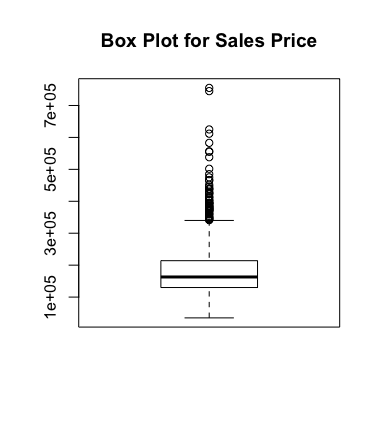
\includegraphics[scale=0.5]{BoxPlotSales}
\\ \caption{\\ Box Plot of Sale Price}
\end{figure}
As we can see, there are a few outliers for the Sales Price, having a value greater than 500,000.
We can compare the boxplot of Sales Price with some of the highly correlated categorical variables and check the outliers with respect to these categories.
\begin{figure}[h!]\centering
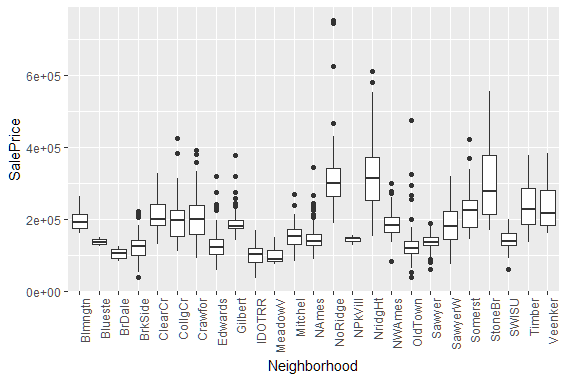
\includegraphics[scale=0.4]{Boxplot1_Neighborhood}
\\ \caption{\\ Box Plot of Neighborhood}
\end{figure}

\begin{figure}[h!]\centering
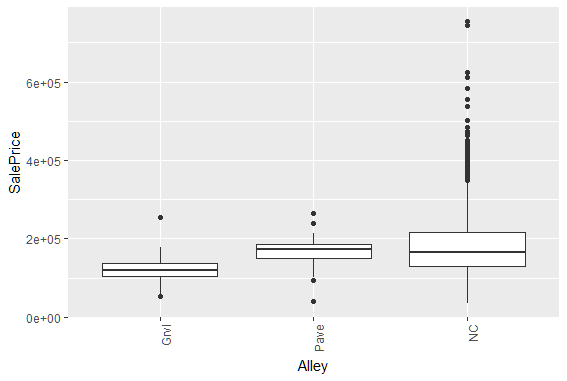
\includegraphics[scale=0.4]{Boxplot2_Alley}
\\ \caption{\\ Box Plot of Alley}
\end{figure}

\begin{figure}[h!]\centering
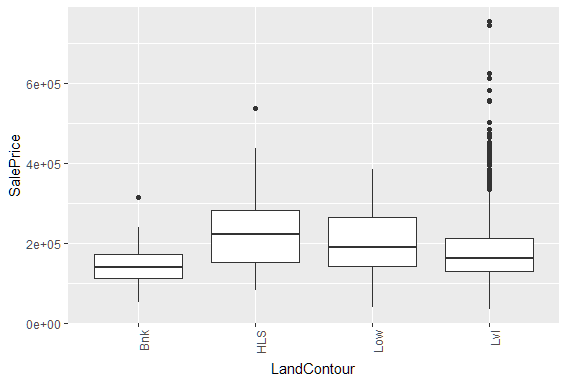
\includegraphics[scale=0.4]{Boxplot3_LandContour}
\\ \caption{\\ Box Plot of LandContour}
\end{figure}

\begin{figure}[h!]\centering
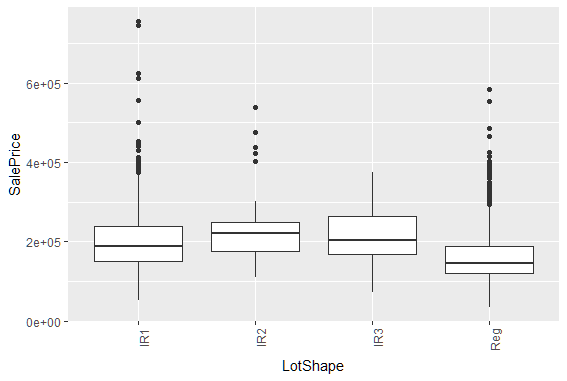
\includegraphics[scale=0.4]{Boxplot4_Lotshape}
\\ \caption{\\ Box Plot of LotShape}
\end{figure}

\subsubsection{Outlier Treatment}
As outliers can affect the overall trend in the data, we will be removing these outliers from the training data. Here we have total 9 values of Sales Price which are greater than 500000, which is just 0.61\%. Hence, we can remove these rows from the data so that there would not be any value that greatly affects the predictions.

\subsubsection{Feature Selection}
\textbf{Feature Selection} starts from an initial set of measured data and builds derived values (features) intended to be informative and non-redundant, facilitating the subsequent learning and generalization steps, and in some cases leading to better human interpretations. Feature selection is related to dimensionality reduction.
When the input data to an algorithm is too large to be processed and it is suspected to be redundant, then it can be transformed into a reduced set of features (also named a features vector). This process is called feature selection \cite{REF:5}.
\\ \\One of the methods for dimensionality reduction is Correlation. Correlation is a statistical technique that can show how strongly a pair of variables are related.
\\ We are using Pearson's Coefficient to measure correlation and this can be done in the \textbf{R} tool using \textbf{cor} function. Below is the graph that shows the correlation among all the numerical attributes.


\begin{figure}[h]\centering
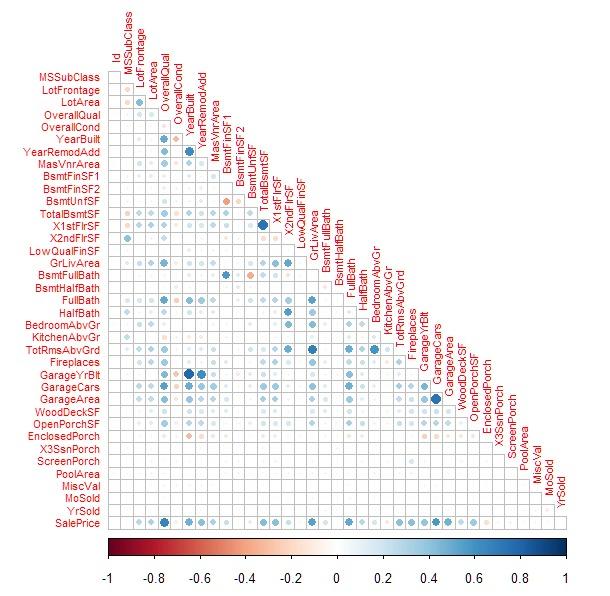
\includegraphics[scale=0.40]{Correlation}
\\ \caption{\\ Correlation Between Variables}
\end{figure}
As it is depicted in the graph, features like OverallQual, GrLiveArea, FullBath, GarageCars are among the few features which have high correlation with the Sales Price.
But the Pearson's coefficient needs the data to be normal and linearly related. In our case, the size of the data is small and just by plotting the graphs it is not easy to predict if the data is normal and features have linear relationship or not. Hence, correlation is not a suitable technique for feature selection for our data.
\\ \\ The method that we have used for feature extraction is using \textbf{Boruta Package} in R tool. The algorithm is designed as a wrapper around a Random Forest classification algorithm. It iteratively removes the features which are proved by a statistical test to be less relevant than random probes. The \textbf{Boruta package} in \textbf{R} provides a convenient interface to the algorithm \cite{REF:7}.
\\ \\Below is the step wise working of \textbf{algorithm} \cite{REF:6}:
\begin{enumerate}[noitemsep]
\item Firstly, it adds randomness to the given data set by creating shuffled copies of all the features (which are called shadow features).
\item Then, it trains a random forest classifier on the extended data set and applies a feature importance measure (the default is Mean Decrease Accuracy) to evaluate the importance of each feature where higher means more important.
\item At every iteration, it checks whether a real feature has a higher importance than the best of its shadow features (i.e. whether the feature has a higher Z score than the maximum Z score of its shadow features) and constantly removes features which are deemed highly unimportant.
\item Finally, the algorithm stops either when all features gets confirmed or rejected or it reaches a specified limit of random forest runs.
\end{enumerate}
The Boruta package was used after the missing values were replaced, as Boruta does not work if we have missing values in data.
After running the Boruta function and plotting the graph we get a list of \textbf{confirmed}, \textbf{tentative} and \textbf{rejected} features.
\begin{figure}[h]
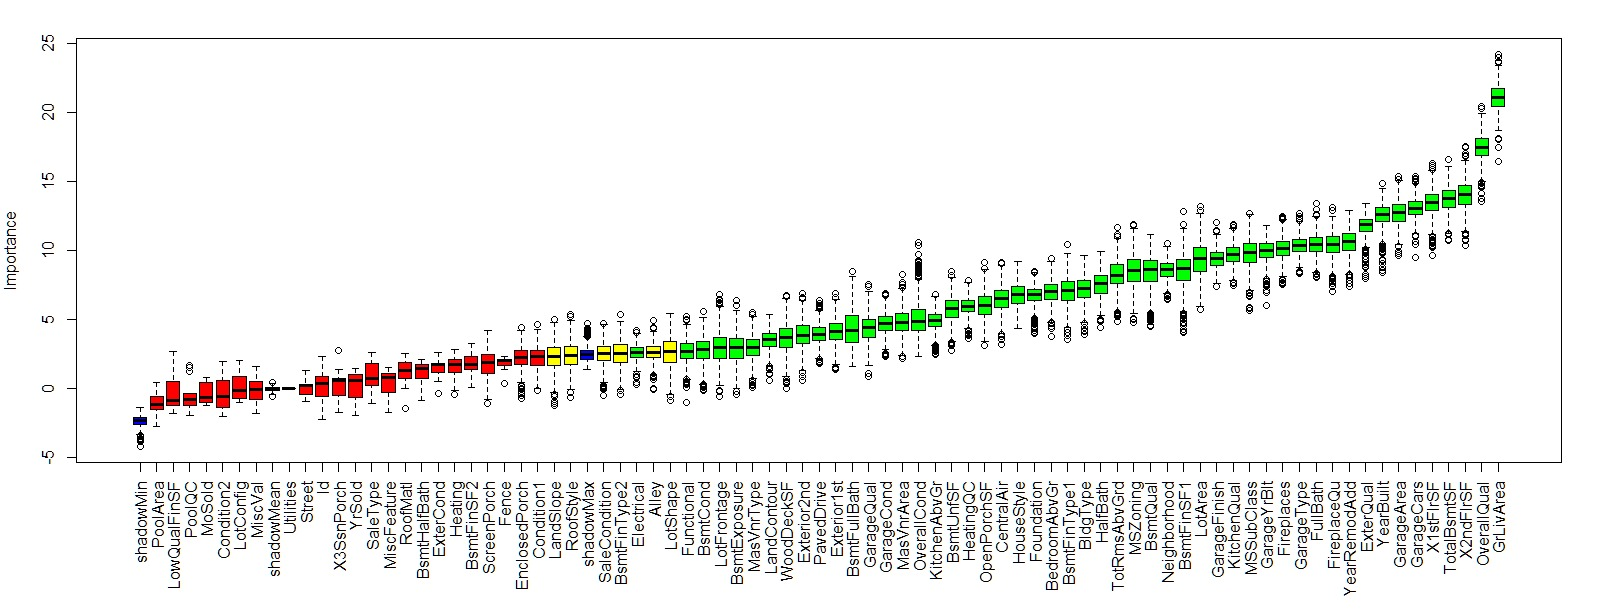
\includegraphics[scale=0.21]{Boruta}
\\ \caption{\\Boruta Plot}
\end{figure}
\\ The \textbf{green} box plots are for the features that have been confirmed, \textbf{yellow} for tentative and \textbf{red} for rejected features.
\subsubsection{Feature Engineering}
After cleaning the data and feature selection based on Boruta we have converted all the categorical attributes into dummy or indicator variables. These dummy variables are created based on the domain of each feature and store either 0 or 1 values, 1 if the value is present for that column or 0 if it is not present. For example, if a categorical feature Alpha has domain \{A, B, C\}, then Alpha would be replaced by three columns named A, B, C. For a particular row, if the value of Alpha is B, then A would be 0, B would be 1 and C would be 0.
\\ These dummy variables tend to have values with more realistic interpretations.


\section{Algorithm and Methodology}
The project mainly deals with using various Regression techniques like \textbf{Linear Regression}, \textbf{Random Forest}, \textbf{Gradient Boosting}, \textbf{Extreme Gradient Boosting} for predictive analysis.
\\ \textbf{What is Regression Analysis?}
\\ Regression analysis is a form of predictive modeling technique which investigates the relationship between a dependent (target) and independent variable(s) (predictor). This technique is used for forecasting, time series modeling and finding the causal effect relationship between the variables \cite{REF:2}. 

\subsection{Regression Techniques}
\begin{enumerate}
\item \textbf{Linear Regression}
\newline A linear regression establishes a relation between a dependent variable (Y) and one or more independent variable(X) using a best fit straight line (also known as "Regression Line").
\\ It is represented by below equation 
\begin{subequations}
\begin{align}
y & = a+bx 
\end{align}

%\begin{figure*}[!]% Using \begin{figure*} makes the figure take up the entire width of the page
%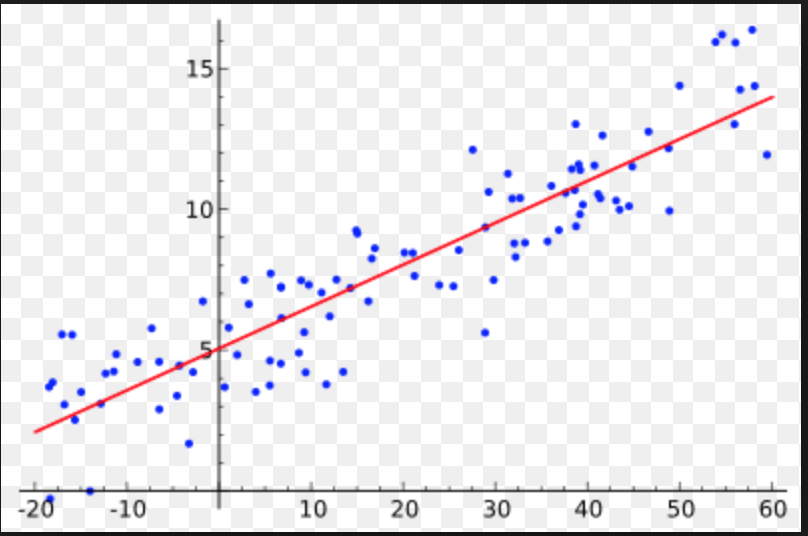
\includegraphics[scale=0.3]{Linearregression}
%\caption{Wide Picture}
%\label{fig:view}
%\end{figure*}

\begin{figure}[h]\centering
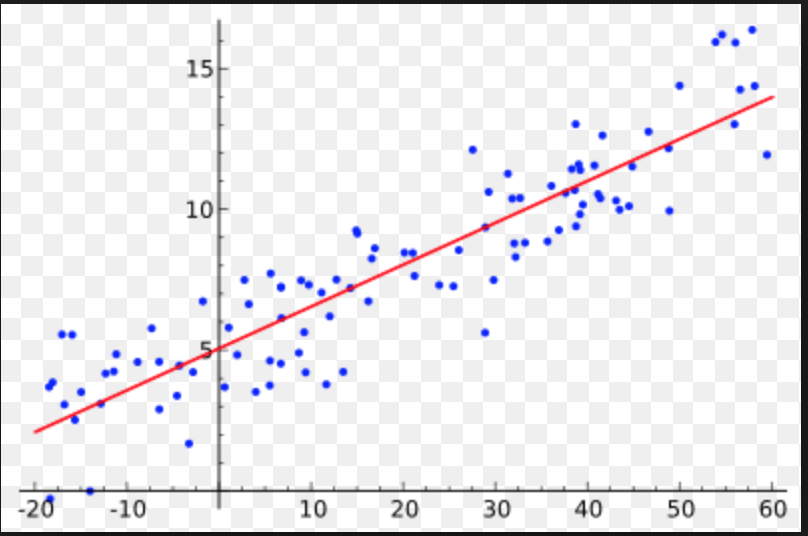
\includegraphics[scale=0.4]{Linearregression}
\\ \caption{\\ Linear Regression Line}
\end{figure}
\end{subequations}
\item \textbf{Random Forest Regression}
\\Random forests or random decision forests are an ensemble learning method for classification, regression and other tasks, that operate by constructing a multitude of decision trees at training time and outputting the class that is mean prediction (regression) of the individual trees \cite{REF:3}.
\item \textbf{Gradient Boosting}
\\Gradient boosting is a machine learning technique for regression and classification problems, which produces a prediction model in the form of an ensemble of weak prediction models, typically decision trees. It builds the model in a stage-wise fashion like other boosting methods do, and it generalizes them by allowing optimization of an arbitrary differentiable loss function \cite{REF:4}.
\item \textbf{Lasso Regression}:
Lasso (least absolute shrinkage and selection operator) is a regression analysis method that performs both variable selection and regularization in order to enhance the prediction accuracy and interpretability of the statistical model it produces.
\end{enumerate}
\subsection{Training of Regression Models}
The method employed to train a prediction model is as follows:
\begin{enumerate}[noitemsep]
\item The given training data is partitioned into two parts. 80\% of the given training data was considered as training data for initial model training and remaining 20\% was considered as test data, for the purpose of calculating the error rates.
\item We use this 80\% data on various regression models.
\item The model was the applied on the 20\% of the data used as test data, and the Sales Price was predicted.
\item The RMSE was calculated using the actual Sales Price and predicted Sales Price.
\item This process was repeated on all regression models.
\end{enumerate}
A 10-fold cross-validation was also applied to decide the optimal number of trees. The figure shows the number of trees used and the average error. We have found that as the number of trees increases, the average error decreases until it converges and then starts increasing again. Other studies have also concluded the same results, that there is a threshold value beyond which there is no advantage in increasing the number of trees.
\begin{figure}[h]\centering
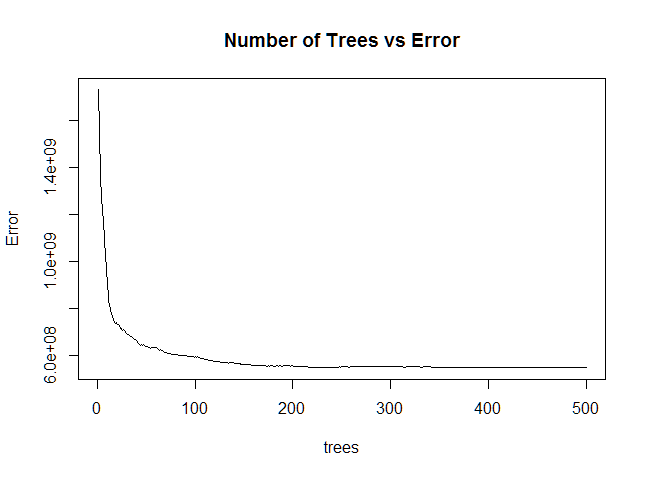
\includegraphics[scale=0.4]{RandomForest}
\\ \caption{\\ Random Forest 10-fold cross-validation}
\end{figure}
\\ \\ Here are some of the parameters that we have optimized for our Random Forest model on the training data:
\\ Number of predictors sampled for splitting at each node: 65
\\ Number of trees: 500
\\ \\ Similarly, for the Gradient Boosting model we have found the optimal values for some parameters on the training data:
\\ Number of trees to fit: 10000
\\ Maximum depth of variable interaction: 15
\\ Learning Rate or step-size reduction: 0.002
\\ Minimum number of observations in tree terminal nodes: 15

%\begin{table}[hbt]
%\caption{Table of Grades}
%\centering
%\begin{tabular}{llr}
%\toprule
%\multicolumn{2}{c}{Name} \\
%\cmidrule(r){1-2}
%First name & Last Name & Grade \\
%\midrule
%John & Doe & $7.5$ \\
%Richard & Miles & $2$ \\
%\bottomrule
%\end{tabular}
%\label{tab:label}
%\end{table}

\section{Experiments and Results}
All the experiments were performed on a machine with two Intel Xeon E5-2650 v2 8-core processors with 32GB of memory, available at Indiana University, Bloomington. We have used R version 3.3.0, R Studio version 0.99.902 for the coding involved in this project.

We have compared the regression models used for predicting the Sales Price of the houses based on the root mean square error (RMSE). Root Mean Square Error is a measure of the quality of an estimator and is the difference between the predicted and observed values.
\\ The formula used for calculating RMSE = $\sqrt{\frac{(predicted-observed)^2}{n}}$
\\ \\After training the regression models, the following values were calculated for RMSE:
\begin{enumerate}[noitemsep] 
\item Linear Regression: 33262.7
\item Simple Trees: 47717.98
\item Random Forest: 28322.66
\item Gradient Boosting: 25877.12
\item Lasso: 27652.61
\item Extreme Gradient Boosting: 30381.65
\end{enumerate}
Also, \textbf{Ensemble Learning} was used to predict the Sales Price of the houses. Ensemble learning creates a predictor or model by combining multiple predictors (from Linear Regression, Random Forest, etc.) to create a stronger overall prediction. An ensemble with two techniques that are more diverse might give much better results than the one with similar techniques involved.
The prediction models for Gradient Boosting and Lasso regression were combined to create the ensemble model here.
The RMSE value for this Ensemble model was calculated to be 21887.75.

After calculating the RMSE values we found out that the ensemble model has the least RMSE among all the predictors used.

The experiment was repeated on the entire training data to train the models again and the Ensemble model was used to predict the final House Prices, as it has the least RMSE out of all the prediction models.



\section{Summary and Conclusions}
The main challenge faced in predicting the Sales Price of the houses was to train the prediction models and find the optimal parameters for each model.

The large number of observations and the attributes present in the training dataset have helped us to analyze and predict the Sales Price of houses correctly, to an extent. We have gained insight about various phases of the Data Mining processes like data preparation, transformation and its validation. It has been found out that a lot of the variation in the Sales Price can be explained by observing the features like GrLivArea, GarageArea, OverallQual, and TotalBsmtSF.

For future work, we would like to train the Extreme Gradient Boosting model more efficiently and also implement other techniques like Ridge Regression, Neural Network.
%------------------------------------------------
\phantomsection
\section*{Acknowledgments} % The \section*{} command stops section numbering

\addcontentsline{toc}{section}{Acknowledgments} % Adds this section to the table of contents
We have put in considerable efforts to reach this stage of the project but it would not have been possible without the continuous guidance and support of many other individuals. We would like to extend our sincere thanks to all of them.
\\ \\ We are highly indebted to our Professor \href{https://www.soic.indiana.edu/all-people/profile.html?profile_id=187}{Mehmet Dalkilic}, for his supervision as well as for providing the necessary resources required for the completion of this project report.
\\ \\ We would also like to thank our Associate Instructor Hasan Kurban for his help and constant support throughout our coursework.


%----------------------------------------------------------------------------------------
%	REFERENCE LIST
%----------------------------------------------------------------------------------------
\phantomsection

\bibliographystyle{unsrt}
\bibliography{report}

%----------------------------------------------------------------------------------------

\end{document}
